\documentclass[11pt,letterpaper,oneside]{article}
\usepackage[top=0.5in,left=1in,right=1in,bottom=1in]{geometry}
%\usepackage[top=0.5in,left=1.8in,right=1.8in,bottom=1in]{geometry}
\usepackage{fancyvrb}
\usepackage{colortbl}
\usepackage[pdftex]{graphicx}
\DeclareGraphicsExtensions{.pdf}
\usepackage{url}
\usepackage{amsmath}

\usepackage{setspace}
\doublespacing

\title{Homework 5}
\author{Dejun Qian}

\date{}

\begin{document}
\maketitle

\begin{description}

\item[Experiment 1:] The sum-squared error is 640310.47. The entropy of the resulting clustering is shown in Table~\ref{tab1}. The average entropy is 0.8988. The accuracy on the test data is 74.09\%. The confusion matrix is shown in Table~\ref{tab2}. We visualize the resulting cluster centers in Figure~\ref{fig1}.

The cluster can recognize most of the digits well. The accuracy is 74.09\%. The visualization results are impressive, most of them look like their associated digits. However, there are no cluster for digit ``9", and the visualization result for digit ``8" is not clear. The accuracy is close to the accuracy from the decision tree method (around 75\%), and less than the accuracy from the naive Bayes classifier (around 90\%).

\begin{table}[th]
\caption{Entropy (K = 10)}
\centering
\begin{tabular*}{0.2\textwidth}{@{\extracolsep{\fill}}cc}
\hline
$Cluster$ & entropy\\ \hline
$C_0$ & 0.00\\
$C_1$ & 0.28\\
$C_2$ & 0.40\\
$C_3$ & 0.00\\
$C_4$ & 0.89\\
$C_5$ & 0.38\\
$C_6$ & 1.54\\
$C_7$ & 0.73\\
$C_8$ & 1.90\\
$C_9$ & 1.68\\
\hline
\end{tabular*}
\label{tab1}
\end{table}

\begin{table}[th]
\caption{Confusion Matrix (K = 10)}
\centering
\begin{tabular*}{0.6\textwidth}{@{\extracolsep{\fill}}ccccccccccc}
\hline
 & 0 & 1 & 2 & 3 & 4 & 5 & 6 & 7 & 8 & 9 \\ \hline
0& 92&  0&  0&  0&  2&  0&  0&  0&  1&  0\\
1& 0& 20&  0&  1&  0&  0&  0&  1& 69&  0\\
2& 0&  0& 81&  4&  0&  0&  0&  3&  6&  0\\
3& 0&   0&   0& 100&   0&   0&   0&   1&   4&   0\\
4& 0&  0&  0&  0& 79&  0&  0&  4&  1&  0\\
5& 0&  1&  0&  6&  2& 69&  1&  0&  9&  0\\
6& 0&  1&  0&  0&  0&  0& 88&  0&  2&  0\\
7& 0&  0&  0&  0&  3&  0&  0& 90&  1&  0\\
8& 0&  0&  0& 13&  1&  1&  0&  0& 73&  0\\
9& 0&  0&  0& 69& 27&  2&  0&  6&  0&  0\\
\hline
\end{tabular*}
\label{tab2}
\end{table}

\begin{figure}
\begin{center}
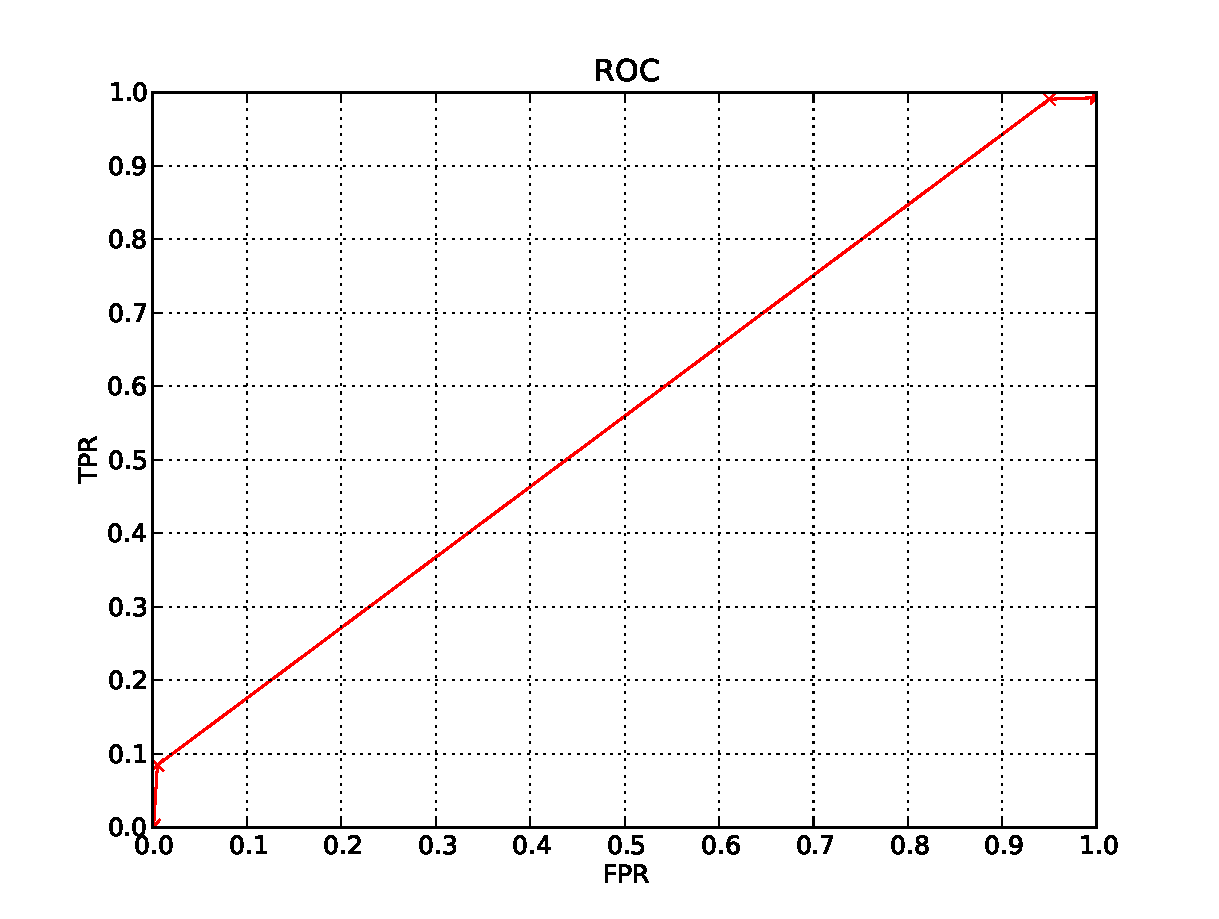
\includegraphics[width=0.95\textwidth]{fig1}
\caption{Visualization (K = 10)}
\label{fig1}
\end{center}
\end{figure}

\item[Experiment 2:] The sum-squared error is 467049.00. The entropy of the resulting clustering is shown in Table~\ref{tab3}. The average entropy is 0.3559. The accuracy on the test data is 90.04\%. The confusion matrix is shown in Table~\ref{tab4}. We visualize the resulting cluster centers in Figure~\ref{fig2}.

Compared to experiment 1, the entropy is lower. The average entropy here is about 40\% of the amount in expriment 1. The maximum entropy in experiment 1 is 1.90, and the maximum entropy here is 1.87. The visualization results look better than the results in experiment 1. The results contain all the digits, and all of them look like their associated digits. The visualization results also show different writing style for the same digit. For example, there are two clusters for the digit ``5", and they look different from each other.

\begin{table}[th]
\caption{Entropy (K = 30)}
\centering
\begin{tabular*}{0.2\textwidth}{@{\extracolsep{\fill}}cc}
\hline
$Cluster$ & entropy\\ \hline
$C_0$ & 0.00\\
$C_1$ & 0.33\\
$C_2$ & 0.00\\
$C_3$ & 0.00\\
$C_4$ & 0.00\\
$C_5$ & 0.24\\
$C_6$ &0.00\\
$C_7$ &0.73\\
$C_8$ &1.31\\
$C_9$ &0.43\\
$C_{10}$ &0.39\\
$C_{11}$ &1.87\\
$C_{12}$ &0.29\\
$C_{13}$ &0.89\\
$C_{14}$ &0.00\\
$C_{15}$ &0.13\\
$C_{16}$ &0.47\\
$C_{17}$ &0.35\\
$C_{18}$ &0.00\\
$C_{19}$ &0.00\\
$C_{20}$ &0.00\\
$C_{21}$ &0.00\\
$C_{22}$ &0.00\\
$C_{23}$ &0.36\\
$C_{24}$ &0.00\\
$C_{25}$ &1.02\\
$C_{26}$ &0.14\\
$C_{27}$ &0.27\\
$C_{28}$ &0.00\\
$C_{29}$ &1.09\\
\hline
\end{tabular*}
\label{tab3}
\end{table}

\begin{table}[th]
\caption{Confusion Matrix (K = 30)}
\centering
\begin{tabular*}{0.6\textwidth}{@{\extracolsep{\fill}}ccccccccccc}
\hline
 & 0 & 1 & 2 & 3 & 4 & 5 & 6 & 7 & 8 & 9 \\ \hline
0& 93&  1&  0&  0&  1&  0&  0&  0&  0&  0\\
1& 0& 78& 12&  0&  0&  0&  0&  0&  0&  1\\
2& 0&  1& 92&  0&  0&  0&  0&  0&  1&  0\\
3& 0&  1&  0& 97&  0&  0&  0&  0&  0&  7\\
4& 0&  0&  0&  0& 79&  0&  0&  5&  0&  0\\
5& 0&  0&  1&  1&  0& 76&  1&  0&  0&  9\\
6& 0&  2&  0&  0&  0&  0& 89&  0&  0&  0\\
7& 0&  0&  3&  0&  0&  0&  0& 91&  0&  0\\
8& 0&  7& 19&  1&  0&  1&  0&  0& 60&  0\\
9& 0&  0&  2&  1&  5&  0&  0&  8&  2& 86\\
\hline
\end{tabular*}
\label{tab4}
\end{table}

\begin{figure}
\begin{center}
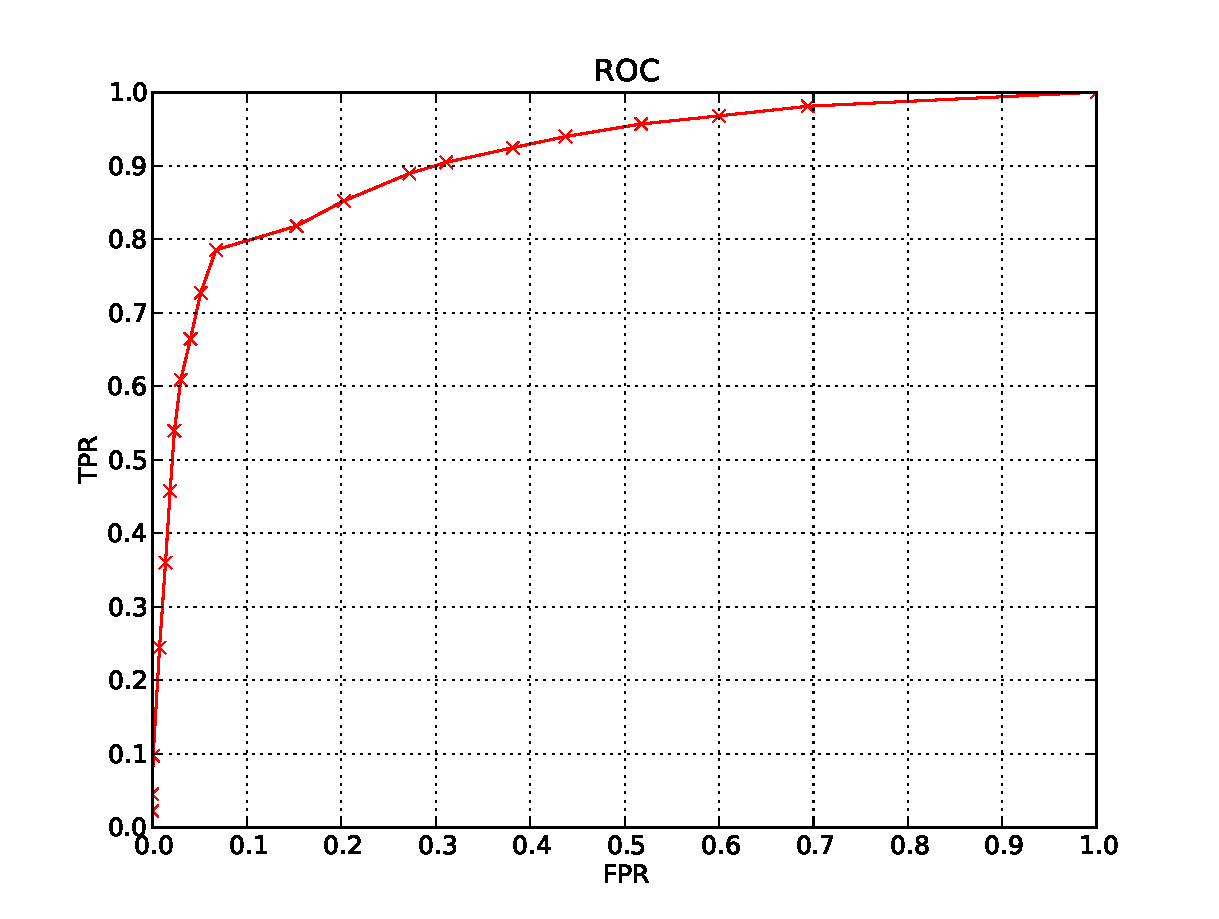
\includegraphics[width=0.95\textwidth]{fig2}
\caption{Visualization (K = 30)}
\label{fig2}
\end{center}
\end{figure}

\end{description}
\end{document}
